\documentclass[tikz,border=12pt]{standalone}
\usepackage{xcolor}
\usepackage{amsmath,amssymb}
\usepackage{times}
\usetikzlibrary{shapes.geometric, arrows.meta, positioning, calc, fit, backgrounds, shadows, fadings}

\definecolor{ieeeBlue}{RGB}{0, 98, 155}
\definecolor{ieeeNavy}{RGB}{0, 40, 85}
\definecolor{ieeeLightBlue}{RGB}{235, 243, 250}
\definecolor{ieeeCyan}{RGB}{0, 163, 196}
\definecolor{ieeeGrayBox}{RGB}{248, 249, 250}
\definecolor{ieeeAccentGreen}{RGB}{0, 138, 90}
\definecolor{ieeeAccentAmber}{RGB}{217, 130, 43}
\definecolor{ieeeAccentRed}{RGB}{198, 40, 40}

\begin{document}
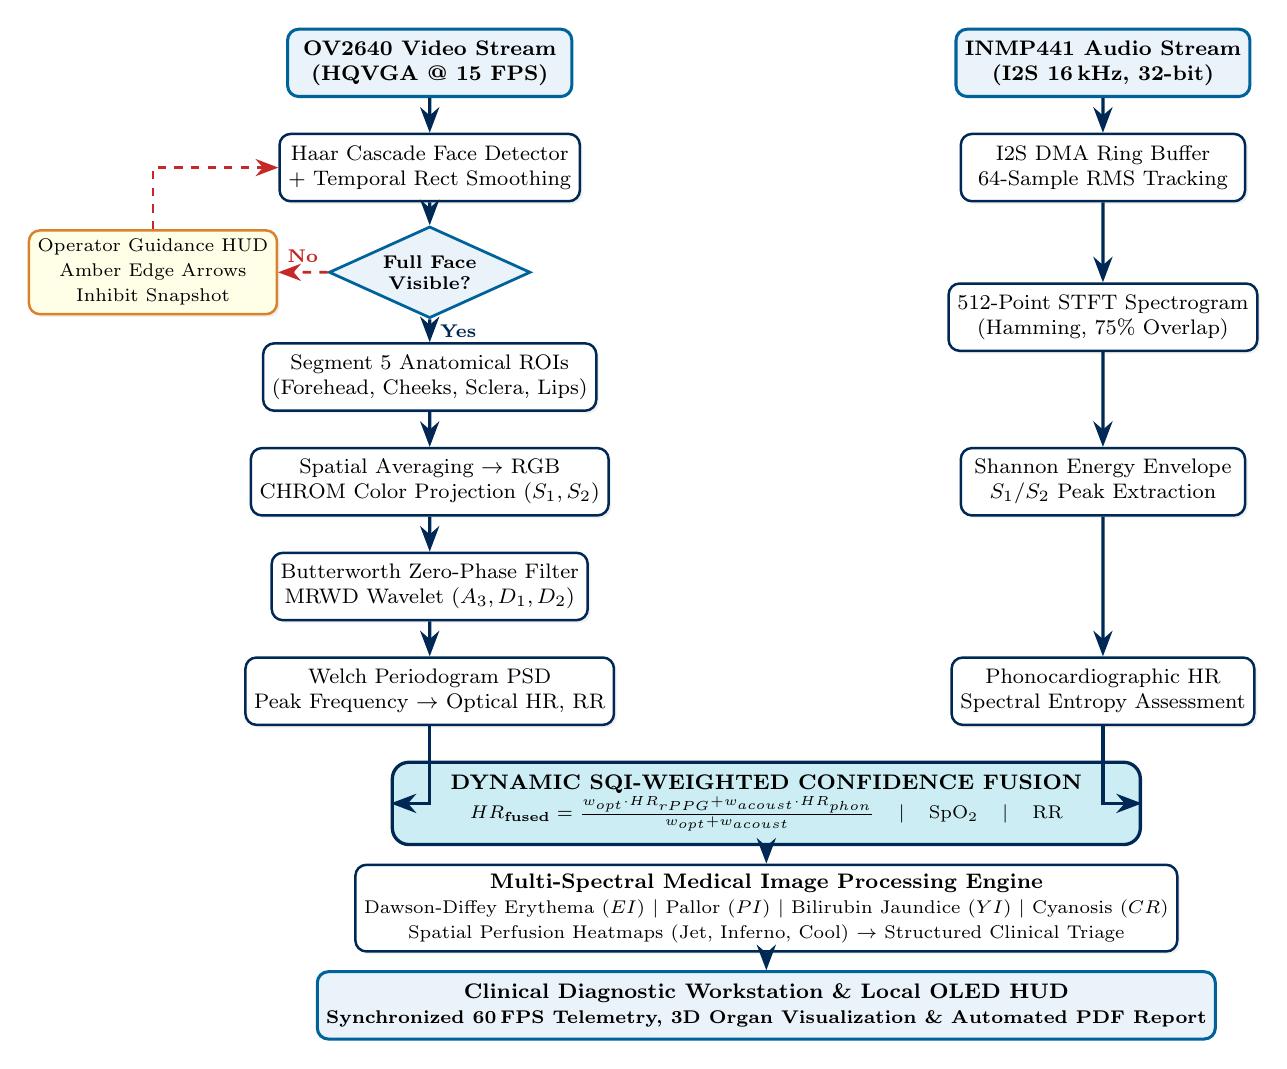
\begin{tikzpicture}[
    scale=0.95, every node/.style={transform shape},
    processNode/.style={draw=ieeeNavy, fill=white, rounded corners=4pt, line width=0.9pt, align=center, font=\footnotesize, minimum height=0.9cm, minimum width=3.8cm, drop shadow={opacity=0.12, shadow xshift=1pt, shadow yshift=-1pt}},
    decisionNode/.style={draw=ieeeBlue, fill=ieeeLightBlue, diamond, aspect=2.2, line width=1.0pt, align=center, font=\scriptsize\bfseries, inner sep=2.0pt},
    sensorNode/.style={draw=ieeeBlue, fill=ieeeLightBlue, rounded corners=4pt, line width=1.1pt, align=center, font=\footnotesize\bfseries, minimum height=0.9cm, minimum width=3.8cm},
    fusionNode/.style={draw=ieeeNavy, fill=ieeeCyan!20, rounded corners=6pt, line width=1.2pt, align=center, font=\footnotesize\bfseries, minimum height=1.1cm, minimum width=10.0cm},
    flowArrow/.style={-{Stealth[scale=1.1]}, line width=1.2pt, color=ieeeNavy},
    rejectArrow/.style={-{Stealth[scale=1.1]}, line width=1.0pt, dashed, color=ieeeAccentRed}
]

% Top Sensors
\node[sensorNode] (camIn) at (-4.5, 7.8) {OV2640 Video Stream\\(HQVGA @ 15 FPS)};
\node[sensorNode] (micIn) at (4.5, 7.8) {INMP441 Audio Stream\\(I2S 16\,kHz, 32-bit)};

% Optical Branch
\node[processNode] (faceDetect) at (-4.5, 6.4) {Haar Cascade Face Detector\\+ Temporal Rect Smoothing};
\node[decisionNode] (fullFaceCheck) at (-4.5, 5.0) {Full Face\\Visible?};
\node[processNode, draw=ieeeAccentAmber, fill=yellow!10, minimum width=3.0cm] (guidance) at (-8.2, 5.0) {
    \scriptsize Operator Guidance HUD\\
    \scriptsize Amber Edge Arrows\\
    \scriptsize Inhibit Snapshot
};
\node[processNode] (roiExtract) at (-4.5, 3.6) {Segment 5 Anatomical ROIs\\(Forehead, Cheeks, Sclera, Lips)};
\node[processNode] (chromProj) at (-4.5, 2.2) {Spatial Averaging $\rightarrow$ RGB\\CHROM Color Projection ($S_1, S_2$)};
\node[processNode] (waveletProc) at (-4.5, 0.8) {Butterworth Zero-Phase Filter\\MRWD Wavelet ($A_3, D_1, D_2$)};
\node[processNode] (welchPsd) at (-4.5, -0.6) {Welch Periodogram PSD\\Peak Frequency $\rightarrow$ Optical HR, RR};

% Acoustic Branch
\node[processNode] (audioBuff) at (4.5, 6.4) {I2S DMA Ring Buffer\\64-Sample RMS Tracking};
\node[processNode] (stftProc) at (4.5, 4.4) {512-Point STFT Spectrogram\\(Hamming, 75\% Overlap)};
\node[processNode] (envelopeProc) at (4.5, 2.2) {Shannon Energy Envelope\\$S_1/S_2$ Peak Extraction};
\node[processNode] (acoustRate) at (4.5, -0.6) {Phonocardiographic HR\\Spectral Entropy Assessment};

% Multimodal Fusion Node
\node[fusionNode] (fusion) at (0, -2.1) {
    DYNAMIC SQI-WEIGHTED CONFIDENCE FUSION\\
    \scriptsize $HR_{\text{fused}} = \frac{w_{opt} \cdot HR_{rPPG} + w_{acoust} \cdot HR_{phon}}{w_{opt} + w_{acoust}} \quad \vert \quad \mathrm{SpO_2} \quad \vert \quad \mathrm{RR}$
};

% Diagnostic Branch
\node[processNode, minimum width=10.0cm] (diagEngine) at (0, -3.5) {
    \textbf{Multi-Spectral Medical Image Processing Engine}\\
    \scriptsize Dawson-Diffey Erythema ($EI$) $\vert$ Pallor ($PI$) $\vert$ Bilirubin Jaundice ($YI$) $\vert$ Cyanosis ($CR$)\\
    \scriptsize Spatial Perfusion Heatmaps (Jet, Inferno, Cool) $\rightarrow$ Structured Clinical Triage
};

% Web Output
\node[sensorNode, minimum width=10.0cm, fill=ieeeLightBlue] (output) at (0, -4.8) {
    \textbf{Clinical Diagnostic Workstation \& Local OLED HUD}\\
    \scriptsize Synchronized 60\,FPS Telemetry, 3D Organ Visualization \& Automated PDF Report
};

% Connectors
\draw[flowArrow] (camIn) -- (faceDetect);
\draw[flowArrow] (faceDetect) -- (fullFaceCheck);
\draw[flowArrow] (fullFaceCheck) -- node[right, font=\scriptsize\bfseries\color{ieeeAccentGreen}] {Yes} (roiExtract);
\draw[rejectArrow] (fullFaceCheck) -- node[above, font=\scriptsize\bfseries\color{ieeeAccentRed}] {No} (guidance);
\draw[rejectArrow] (guidance) |- (faceDetect);
\draw[flowArrow] (roiExtract) -- (chromProj);
\draw[flowArrow] (chromProj) -- (waveletProc);
\draw[flowArrow] (waveletProc) -- (welchPsd);

\draw[flowArrow] (micIn) -- (audioBuff);
\draw[flowArrow] (audioBuff) -- (stftProc);
\draw[flowArrow] (stftProc) -- (envelopeProc);
\draw[flowArrow] (envelopeProc) -- (acoustRate);

\draw[flowArrow] (welchPsd.south) |- (fusion.west);
\draw[flowArrow] (acoustRate.south) |- (fusion.east);

\draw[flowArrow] (fusion) -- (diagEngine);
\draw[flowArrow] (diagEngine) -- (output);

\end{tikzpicture}
\end{document}
